
\chapter{Frameworks}
\newpage

\section{Documenting Attacks and Adversaries}
\begin{itemize}
  \item Documentation is today still text based (think emails, incident reports in Word/PDF, news articles)
  \item Framework needed to have a common description language
  \item “Cyber Kill Chain”, Developed by Lockheed Martin
  \item “Diamond Model”, Developed by Caltagirone, Pendergast, and Betzis
  \item STIX/TAXII, Sponsored by the U.S. Department of Homeland Security are heavily supported by MITRE corporation
  \item MISP Malware Information Sharing Project, MISP is an open source software
  \item MITRE “ATT\&CK”, Developed by MITREM
\end{itemize}

\subsection{Cyber Kill Chain}
\textbf{Old}
\begin{center}
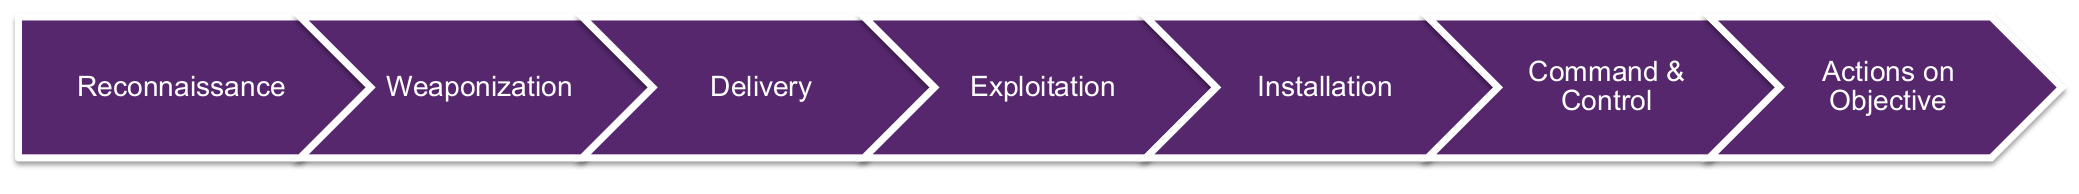
\includegraphics[width=\textwidth]{resources/09-cyber-kill-chain.png}
Here's a more structured LaTeX explanation with the requested elements:
\end{center}

\subsection{Cyber Kill Chain}
The Cyber Kill Chain is a cybersecurity framework developed by Lockheed Martin that models cyber attacks as a sequence of steps. It helps security teams understand and defend against advanced persistent threats (APTs) by breaking down the attack process.

\subsubsection{Purpose}
It enables organizations to:
\begin{itemize}
    \item Identify and stop attacks at each stage
    \item Develop specific countermeasures
    \item Map security controls and gaps
\end{itemize}

\subsubsection{Framework Stages}
\begin{description}
    \item[Reconnaissance] Harvesting email addresses, conference information, social relationships
    \item[Weaponization] Coupling exploit with backdoor into deliverable payload
    \item[Delivery] Transmission of weapon via email, web, USB
    \item[Exploitation] Triggering the attacker's code (e.g., exploiting an application vulnerability)
    \item[Installation] Installing malware, backdoor, or other persistence mechanism
    \item[Command \& Control (C2)] Establishing a command channel for remote manipulation
    \item[Actions on Objectives] Accomplishing the original goals (e.g., data exfiltration)
\end{description}

\subsubsection{Example IoCs per Stage}
Consider a spear-phishing attack:
\begin{itemize}
    \item \textbf{Reconnaissance:} OSINT tool connections from IP 192.0.2.1
    \item \textbf{Weaponization:} Maldoc hash: 5f2de... (SHA256)
    \item \textbf{Delivery:} Email from spoofed domain @company-updates.com
    \item \textbf{Exploitation:} CVE-2021-44228 attempts in web logs
    \item \textbf{Installation:} New service creation "svchost32.exe"
    \item \textbf{C2:} Beacon to domain evil-c2.com every 60 seconds
    \item \textbf{Actions:} Large outbound data transfers to 198.51.100.2
\end{itemize}

\subsection{Unified Kill Chain (UKC)}

\textbf{Improved $\rightarrow$ Unified Kill Chain}

\begin{center}
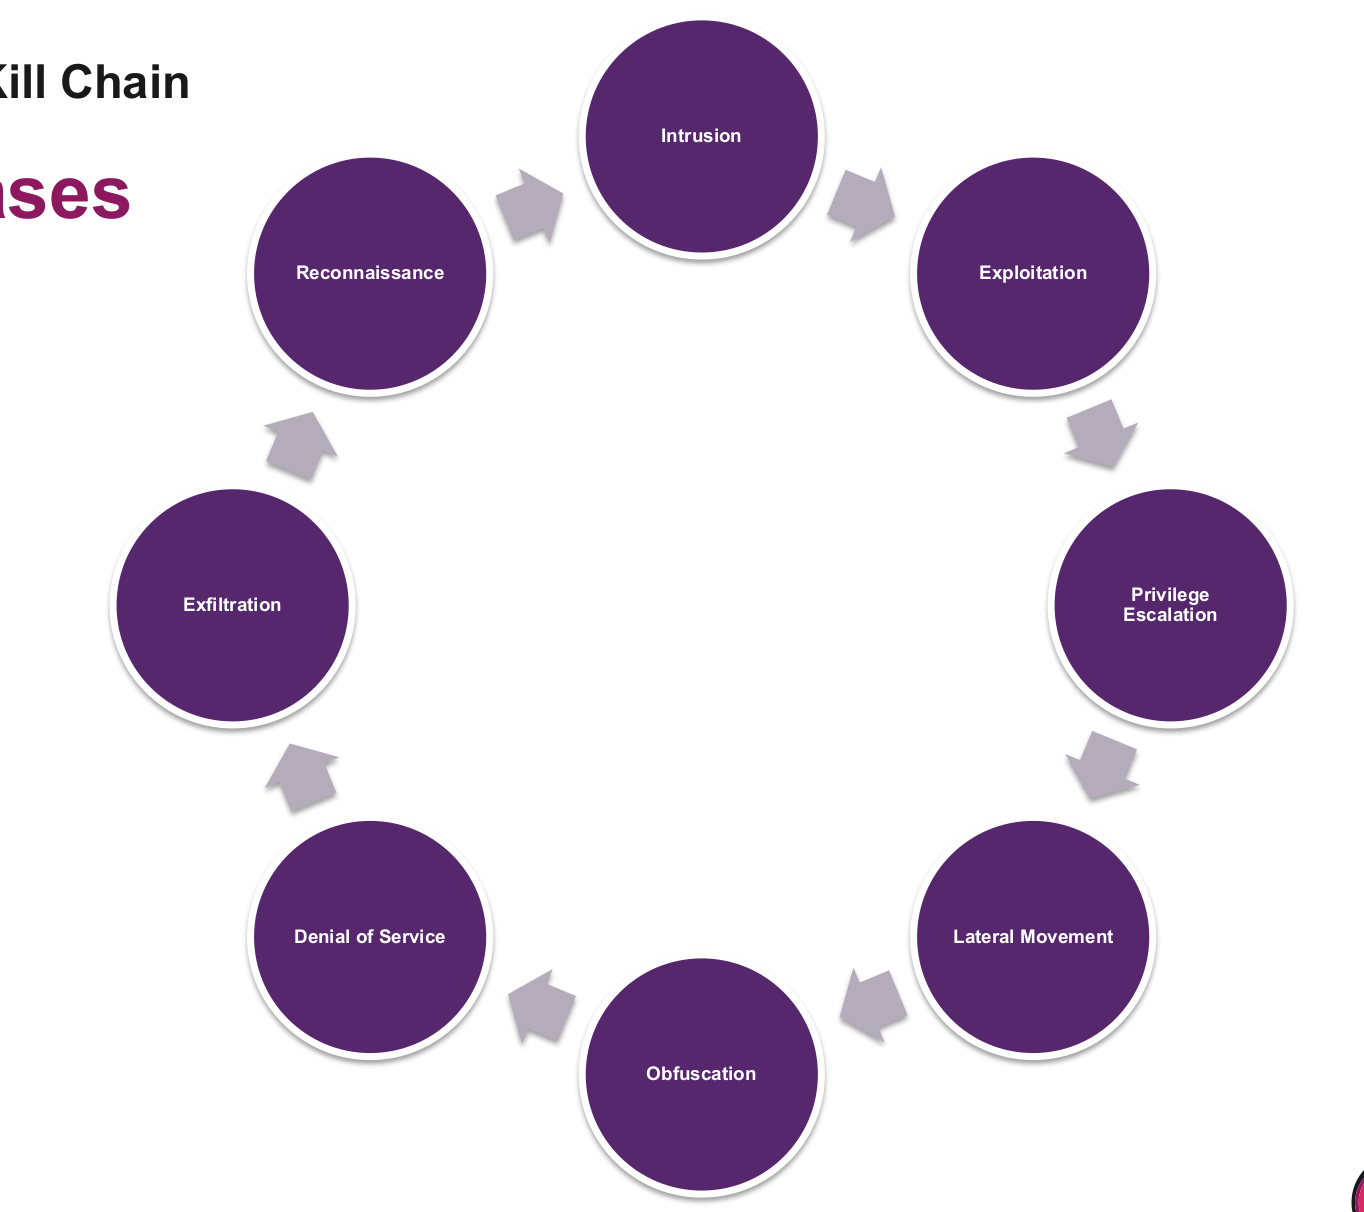
\includegraphics[width=\textwidth]{resources/09-cyber-kill-chain-improved.png}
\end{center}

The Unified Kill Chain represents a modern, cyclical approach to understanding cyber attacks. Unlike the traditional linear models, it emphasizes the interconnected nature of attack phases.

\subsubsection{Overview}
A comprehensive framework that models cyber attacks as a continuous cycle consisting of eight primary phases:

\begin{description}
   \item[Reconnaissance] Initial information gathering and footprinting
   \item[Intrusion] Establishing initial access to the target system
   \item[Exploitation] Leveraging vulnerabilities for system access
   \item[Privilege Escalation] Gaining elevated system permissions
   \item[Lateral Movement] Expanding access across the network
   \item[Obfuscation] Hiding malicious activities and presence
   \item[Denial of Service] Optional phase for system disruption
   \item[Exfiltration] Data theft and extraction
\end{description}

\subsubsection{Key Characteristics}
\begin{itemize}
   \item Cyclical rather than linear progression
   \item Phases can occur in varying orders
   \item Emphasizes post-exploitation activities
   \item Includes defensive evasion explicitly
   \item Adaptable to various attack scenarios
\end{itemize}

\subsubsection{Example Indicators}
Attack indicators for different phases:
\begin{itemize}
   \item \textbf{Reconnaissance:} Port scans from 192.0.2.1
   \item \textbf{Intrusion:} Failed login attempts from external IPs
   \item \textbf{Exploitation:} Unusual process spawning from Office apps
   \item \textbf{Privilege Escalation:} Use of mimikatz.exe
   \item \textbf{Lateral Movement:} SMB connections between workstations
   \item \textbf{Obfuscation:} Cleared Windows Event Logs
   \item \textbf{Denial of Service:} Traffic spike to 10GB/s
   \item \textbf{Exfiltration:} Large outbound transfers to unknown IPs
\end{itemize}


\subsection{Diamond Model of Intrusion Analysis}
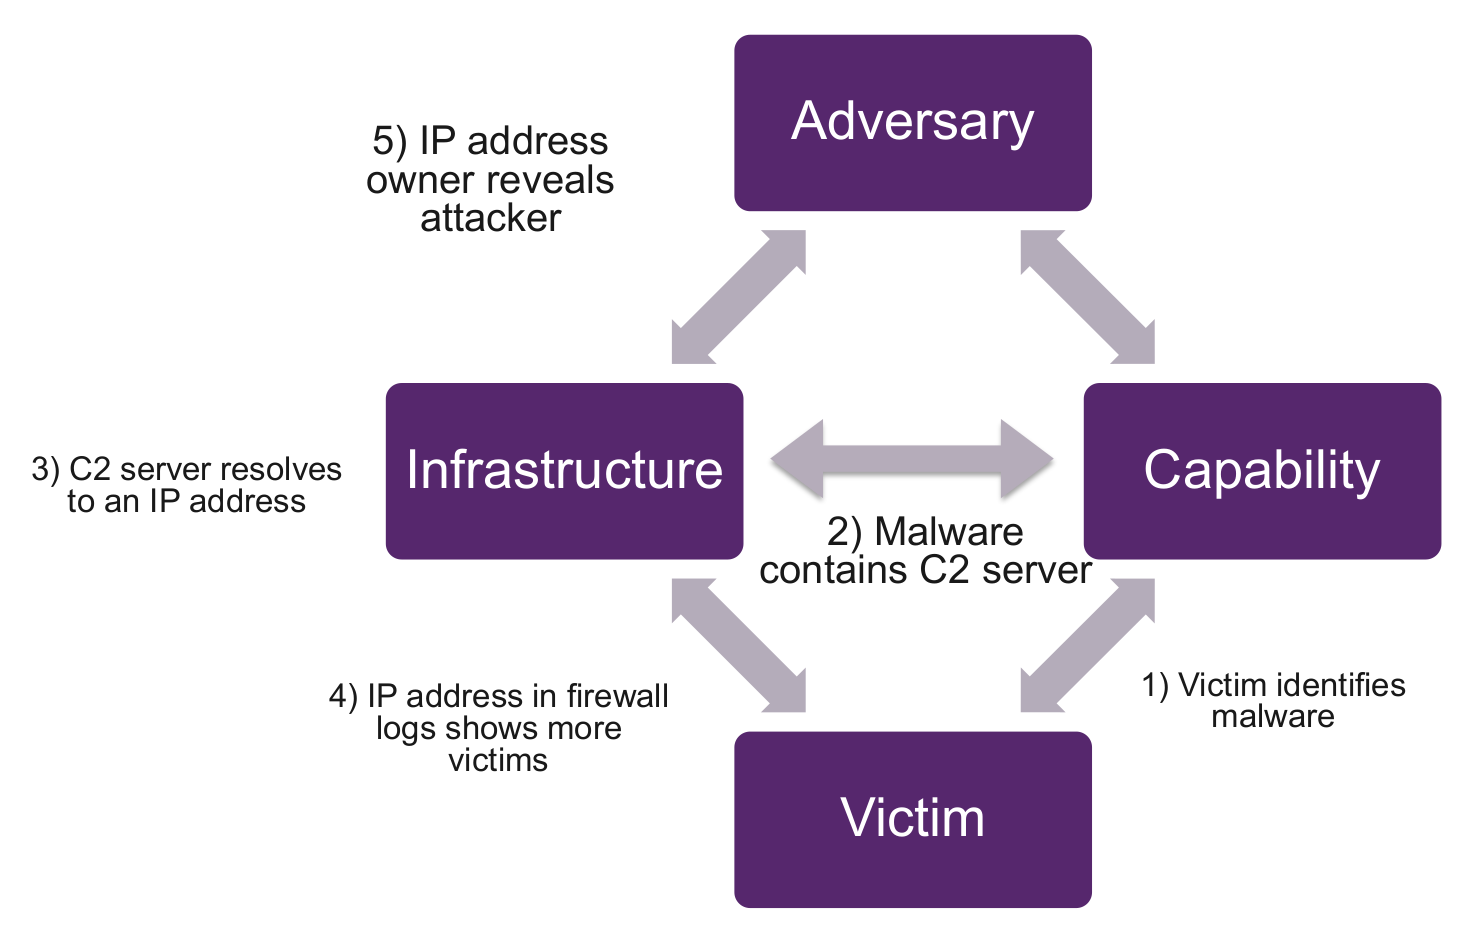
\includegraphics[width=\textwidth]{resources/09-diamond-model.png}

The Diamond Model is a framework for analyzing cyber intrusions through four core interconnected elements forming a diamond shape.

\subsubsection{Core Components}
\begin{description}
    \item[Adversary] The malicious actor conducting the operation
    \item[Capability] Tools and techniques used (malware, exploits)
    \item[Infrastructure] Systems used to deliver capabilities (C2 servers, domains)
    \item[Victim] The target of the intrusion
\end{description}

\subsubsection{Component Relationships}
The model demonstrates key relationships in an intrusion:

\begin{enumerate}
    \item \textbf{Victim $\rightarrow$ Capability}
    \begin{itemize}
        \item Victim identifies malicious software
        \item Initial discovery of attack artifacts
    \end{itemize}
    
    \item \textbf{Capability $\rightarrow$ Infrastructure}
    \begin{itemize}
        \item Malware analysis reveals C2 server details
        \item Understanding of attacker infrastructure
    \end{itemize}
    
    \item \textbf{Infrastructure Analysis}
    \begin{itemize}
        \item C2 domain resolves to specific IP addresses
        \item Infrastructure mapping and analysis
    \end{itemize}
    
    \item \textbf{Infrastructure $\rightarrow$ Victim}
    \begin{itemize}
        \item Firewall logs reveal additional victims
        \item Campaign scope identification
    \end{itemize}
    
    \item \textbf{Infrastructure $\rightarrow$ Adversary}
    \begin{itemize}
        \item IP ownership unmasks attacker identity
        \item Attribution through infrastructure analysis
    \end{itemize}
\end{enumerate}

\subsubsection{Model Applications}
\begin{itemize}
    \item Incident Response planning
    \item Threat Intelligence analysis
    \item Campaign tracking
    \item Attribution efforts
    \item Defensive planning
\end{itemize}

\subsection{}
\begin{center}
\end{center}

\subsection{STIX \& TAXII Framework}
STIX and TAXII are complementary standards for describing and sharing cyber threat intelligence (CTI).

\subsubsection{STIX Overview}
A standardized language for describing cyber threat intelligence:

\begin{description}
    \item[STIX Objects] Core components for describing threats:
    \begin{itemize}
        \item \textbf{Indicators}: IPs, hashes, domains
        \item \textbf{Observables}: Events, artifacts
        \item \textbf{Incidents}: Security events
        \item \textbf{Tactics}: MITRE ATT\&CK mappings
        \item \textbf{Threat Actors}: Adversary groups
        \item \textbf{Campaign}: Sets of activities
    \end{itemize}
\end{description}

\subsubsection{TAXII Overview}
Transport protocol for sharing STIX data:

\begin{description}
    \item[Core Services]
    \begin{itemize}
        \item \textbf{Collection}: Data repositories
        \item \textbf{Channel}: Real-time streams
        \item \textbf{API Root}: Service discovery
    \end{itemize}
    
    \item[Sharing Models]
    \begin{itemize}
        \item \textbf{Hub}: Central source
        \item \textbf{Source/Subscriber}: Push/pull model
        \item \textbf{Peer-to-Peer}: Direct sharing
    \end{itemize}
\end{description}

\subsubsection{Implementation Example}
\begin{verbatim}
{
    "type": "indicator",
    "spec_version": "2.1",
    "id": "indicator--8e2e2d2b-17d4-4cbf-938f-98ee46b3cd3f",
    "created": "2024-01-12T04:31:19.743Z",
    "modified": "2024-01-12T04:31:19.743Z",
    "indicator_types": ["malicious-activity"],
    "pattern": "[ipv4-addr:value = '198.51.100.1']",
    "pattern_type": "stix",
    "valid_from": "2024-01-12T04:31:19.743Z"
}
\end{verbatim}

Key benefits:
\begin{itemize}
  \item Standardized threat sharing
  \item Automated processing
  \item Vendor-agnostic format
  \item Community adoption
  \item Machine-readable format
\end{itemize}

\subsection{}
\subsection{MISP - Malware Information Sharing Platform}
An open-source threat intelligence platform for sharing, storing, and correlating threat indicators.

\begin{itemize}
  \item A threat intelligence platform for gathering, sharing, storing and correlating Indicators of Compromise (IOC) of targeted attacks, threat intelligence, financial fraud information, vulnerability information or even counter-terrorism information.
  \begin{itemize}
    \item Store your IOCs in a structured manner, and thus enjoy the correlation, automated exports for IDS, or SIEM, in STIX or OpenIOC and synchronize to other MISP instances
    \item Make it easier for you to share with, but also to receive from trusted partners and trust-groups
  \end{itemize}
  \item Core development by CIRCL, the Computer Incident Response Center in Luxembourg
  \begin{itemize}
    \item Accepts commits and requests via GitHub
  \end{itemize}
\end{itemize}

\subsubsection{Core Features}
\begin{description}
    \item[Events] Core unit of information:
    \begin{itemize}
        \item Incidents
        \item Malware analysis
        \item Threat intelligence reports
        \item Vulnerability data
    \end{itemize}
    
    \item[Attributes] Technical details within events:
    \begin{itemize}
        \item IP addresses
        \item Domain names
        \item File hashes
        \item Threat actors
        \item Tools
    \end{itemize}
    
    \item[Taxonomies] Classification schemas:
    \begin{itemize}
        \item MITRE ATT\&CK
        \item Traffic Light Protocol (TLP)
        \item False Positive Classification
    \end{itemize}
\end{description}

\subsubsection{Sharing Features}
\begin{itemize}
    \item \textbf{Synchronization}: Between MISP instances
    \item \textbf{Export}: STIX, CSV, OpenIOC, Text
    \item \textbf{API}: RESTful and Python PyMISP
    \item \textbf{Automation}: Feeds and automation tasks
\end{itemize}

\subsubsection{Integration Capabilities}
Common integrations include:
\begin{itemize}
    \item \textbf{SIEM}: Splunk, ELK
    \item \textbf{IDS}: Suricata, Snort
    \item \textbf{Analyzers}: VirusTotal, YARA
    \item \textbf{Ticketing}: TheHive, RTIR
\end{itemize}

\subsubsection{MISP Published Standards}
\begin{itemize}
  \item MISP core format: used to exchange indicators and threat information between MISP instances
  \item MISP object template format: describes a simple JSON format to represent the various templates used to construct MISP objects
  \item MISP taxonomy format: describes a simple JSON format to represent machine tag vocabularies
  \item MISP galaxy format: simple JSON format to represent galaxies and clusters that can be attached to MISP events or attributes
  \item SightingDB format: to give automated context to a given Attribute by counting occurrences and tracking times of observability
\end{itemize}

\begin{lstlisting}[language=JSON]
{
    "Event": {
        "id": "1",
        "org_id": "1",
        "date": "2024-01-12",
        "threat_level_id": "2",
        "info": "Phishing Campaign",
        "published": false,
        "uuid": "50c..",
        "attribute_count": "8",
        "analysis": "2",
        "timestamp": "1234567890",
        "distribution": "1",
        "proposal_email_lock": false,
        "locked": false,
        "publish_timestamp": "1234567890",
        "sharing_group_id": "0",
        "disable_correlation": false,
        "extends_uuid": ""
    }
}
\end{lstlisting}

\subsection{MITRE ATT\&CK Framework}
A comprehensive knowledge base of adversary tactics and techniques based on real-world observations.

\subsubsection{Core Components}
\begin{description}
    \item[Tactics] Categories representing adversary's tactical goals:
    \begin{itemize}
        \item Initial Access
        \item Execution
        \item Persistence
        \item Privilege Escalation
        \item Defense Evasion
        \item Credential Access
        \item Discovery
        \item Lateral Movement
        \item Collection
        \item Exfiltration
        \item Command and Control
        \item Impact
    \end{itemize}
    
    \item[Techniques] Specific methods to achieve tactical goals:
    \begin{itemize}
        \item Detailed descriptions
        \item Detection guidance
        \item Mitigation strategies
        \item Related procedures
    \end{itemize}
    
    \item[Sub-techniques] More specific variants of techniques:
    \begin{itemize}
        \item Detailed implementations
        \item Platform-specific methods
        \item Variant procedures
    \end{itemize}
\end{description}

\subsubsection{Matrix Structure}
\begin{itemize}
    \item \textbf{Enterprise ATT\&CK}
    \begin{itemize}
        \item Windows, Linux, macOS
        \item Cloud platforms
        \item Network infrastructure
    \end{itemize}
    
    \item \textbf{Mobile ATT\&CK}
    \begin{itemize}
        \item Android
        \item iOS
    \end{itemize}
    
    \item \textbf{ICS ATT\&CK}
    \begin{itemize}
        \item Industrial Control Systems
        \item Operational Technology
    \end{itemize}
\end{itemize}

\subsubsection{Practical Applications}
\begin{itemize}
    \item Threat Intelligence mapping
    \item Security gap analysis
    \item Red team planning
    \item Blue team detection strategies
    \item Risk assessment
    \item Security architecture design
\end{itemize}



\subsubsection{Example Technique}
\begin{lstlisting}[language=JSON]
{
    "technique_id": "T1059",
    "name": "Command and Scripting Interpreter",
    "tactic": "Execution",
    "platforms": ["Windows", "macOS", "Linux"],
    "sub_techniques": [
        "PowerShell",
        "Python",
        "Windows Command Shell"
    ],
    "detection": "Process monitoring, command-line logging"
}
\end{lstlisting}

\subsection{ATT\&CK Threat Actor Flash Card}
A standardized format for documenting threat actor profiles in the MITRE ATT\&CK framework.

\subsubsection{Core Components}
\begin{description}
    \item[Threat Actor ID] Unique identifier (e.g., G0008)
    
    \item[Associated Groups] Alternative names/aliases:
    \begin{itemize}
        \item APT names (e.g., APT28)
        \item Industry names (e.g., FANCY BEAR)
        \item Country references (if attributed)
    \end{itemize}
    
    \item[Techniques Used] Documented ATT\&CK techniques:
    \begin{itemize}
        \item Commonly used TTPs
        \item Signature moves
        \item Tool preferences
    \end{itemize}
    
    \item[Target Industries]
    \begin{itemize}
        \item Sectors targeted
        \item Geographic focus
        \item Types of victims
    \end{itemize}
    
    \item[Attributed Malware]
    \begin{itemize}
        \item Custom tools
        \item Known malware families
        \item Specific variants
    \end{itemize}
\end{description}

\subsubsection{Example Flash Card}
\begin{lstlisting}[language=JSON]
{
    "id": "G0008",
    "name": "Example Group",
    "aliases": ["APT28", "FANCY BEAR"],
    "techniques": ["T1059", "T1078", "T1110"],
    "tools": ["X-Agent", "X-Tunnel"],
    "targets": ["Government", "Defense"],
    "description": "Active since 2004..."
}
\end{lstlisting}

\subsubsection{Word of Cuation}
\begin{itemize}
  \item It is also important to understand what ATT\&CK is not
  \begin{itemize}
    \item Not a checklist: do not use this as a simple “can we detect this”, but understand the attack, translate it into your environment, compare to existing controls
    \item Not a bingo-card: do not mark what you can cover
    \item Documenting every possible attack: ATT\&CK documents the known TTPs: when you document your own attacks/campaigns, you realise that you have more information about an attacker than what ATT\&CK currently publicly describes
    \item Static, final list: the ATT\&CK matrixes are improved or modified regularly and now include PRE-ATT\&CK (preparation attackers perform) and Mobile
  \end{itemize}
\end{itemize}

\subsection{ATT\&ck vs. Kill Chain}
\begin{itemize}
  \item The tactics allow you to show the lifecycle/progress of an attack inside your enterprise
  \item Similar to what we saw with the Cyber Kill Chain
    \item Some tactic are equal or very similar (intrusion and initial access, privilege escalation, exfiltration), others do not exists in one or the other (denial of service, discovery)
  \item The kill chain is more linear, as an attacker you move from left to right
  \item ATT\&CK is more graph-like, move from left to right but also within the tactics up and down
  \item Defenders need to think in graphs, not in lists
\end{itemize}


\subsection{MITRE ATT\&CK Categories and Hunting Potential}

\subsubsection{Categories by Hunting Potential}
\begin{description}
   \item[High Value (4)] Most reliable to detect:
   \begin{itemize}
       \item Command and Control
       \item Exfiltration
       \item Lateral Movement
       \item Persistence
   \end{itemize}

   \item[Good Value (3)] Good detection rate:
   \begin{itemize}
       \item Credential Access
       \item Discovery 
       \item Execution
       \item Collection
   \end{itemize}

   \item[Moderate Value (2)] More difficult to detect:
   \begin{itemize}
       \item Initial Access
       \item Privilege Escalation
       \item Impact
   \end{itemize}

   \item[Low Value (1)] Hardest to detect:
   \begin{itemize}
       \item Defense Evasion
   \end{itemize}
\end{description}

\subsubsection{Hunting Focus Areas}
Based on the potential values:

\begin{description}
   \item \textbf{Primary Focus} (4):
   \begin{itemize}
       \item Monitor C2 traffic patterns
       \item Track data movement
       \item Watch network connections
       \item Check persistence mechanisms
   \end{itemize}
   
   \item \textbf{Secondary Focus} (3):
   \begin{itemize}
       \item Monitor credential usage
       \item Track system discovery
       \item Watch process execution
   \end{itemize}
   
   \item \textbf{Supplementary} (2-1):
   \begin{itemize}
       \item Initial access alerts
       \item Privilege changes
       \item Evasion attempts
   \end{itemize}
\end{description}

\section{exercise}
